\section{Boolean Set-Operations on Linear Polygons\label{bso_sec:bso_lin}}
% =================================================

The basic library of \cgal\ includes the \ccc{Polygon_2<Kernel,Container>}
class-template that represents a linear polygon in the plane. The
polygon is represented by its vertices stored in a container of
objects of type \ccc{Kernel::Point_2}. The polygon edges are line
segments (\ccc{Kernel::Segment_2} objects) between adjacent points in
the container. By default, the \ccc{Container} is a vector of
\ccc{Kernel::Point_2} objects.

The following function demonstrates how to use the basic access
functions of the \ccc{Polygon_2} class. It accepts a polygon $P$ and
prints it in a readable format:
\begin{alltt}
template<class Kernel, class Container>
void print_polygon (const CGAL::Polygon_2<Kernel, Container>& P)
\{
  typename CGAL::Polygon_2<Kernel, Container>::Vertex_const_iterator  vit;

  std::cout << "[ " << P.size() << " vertices:";
  for (vit = P.vertices_begin(); vit != P.vertices_end(); ++vit)
    std::cout << " (" << *vit << ')';
  std::cout << " ]" << std::endl;
\}
\end{alltt}

In this section we use the term {\em polygon} to indicate a
\ccc{Polygon_2} instance, namely, a polygon having linear
edges. General polygons are only discussed in
Section~\ref{bso_sec:bso_gen}.

The basic components of our package are the free (global) functions
\ccc{complement()} that accepts a single \ccc{Polygon_2} object, and
\ccc{intersection()}, \ccc{join()},\footnote{The function that
computes the union of two polygons is called \ccc{join()}, since
the word \ccc{union} is reserved in \CC.} \ccc{difference()},
\ccc{symmetric_difference()} and the predicate \ccc{do_intersect()}
that accept two \ccc{Polygon_2} objects as their input. We explain how
these functions should be used through several examples in the
following sections.

% ~~~~~~~~~~~~~~~~~~~~~~~~~~~~~~~
\subsubsection*{A Simple Example}
% ~~~~~~~~~~~~~~~~~~~~~~~~~~~~~~~

\lcTex{%
  \setlength{\BooleanSetOpsWidthRight}{1.4cm}
  \setlength{\BooleanSetOpsWidthLeft}{\BooleanSetOpsWidthLineReal}
  \addtolength{\BooleanSetOpsWidthLeft}{-\BooleanSetOpsWidthRight}
  \begin{minipage}{\BooleanSetOpsWidthLeft}
}
\label{fig:example}
\begin{ccHtmlOnly}
  <p><center>
    <img src="./fig/triangles.gif" border=0 alt="Two triangles" align=right>
  </center>
\end{ccHtmlOnly}
Testing whether two polygons intersect results with a Boolean value, 
and does not require any additional data beyond the provision of the 
two input polygons. The example listed below tests whether the two
triangles depicted on the right intersect. It uses, as do the other
example programs in this chapter, the auxiliary header file
\ccc{bso_rational_nt.h}, which defines the type \ccc{Number_type} as
{\sc Gmp}'s rational number-type (\ccc{CGAL::Gmpq}), or as the
number type \ccc{Quotient<MP_Float>} that is included in the support
library of \cgal, based on whether the {\sc Gmp} library is installed
or not. It also uses the function \ccc{print_polygon.h} listed above,
which is located in the header file \ccc{print_utils.h}.
\lcTex{%
  \end{minipage}\hspace{\BooleanSetOpsMinipageSpace}
  \begin{minipage}{\BooleanSetOpsWidthRight}
    \begin{center}
    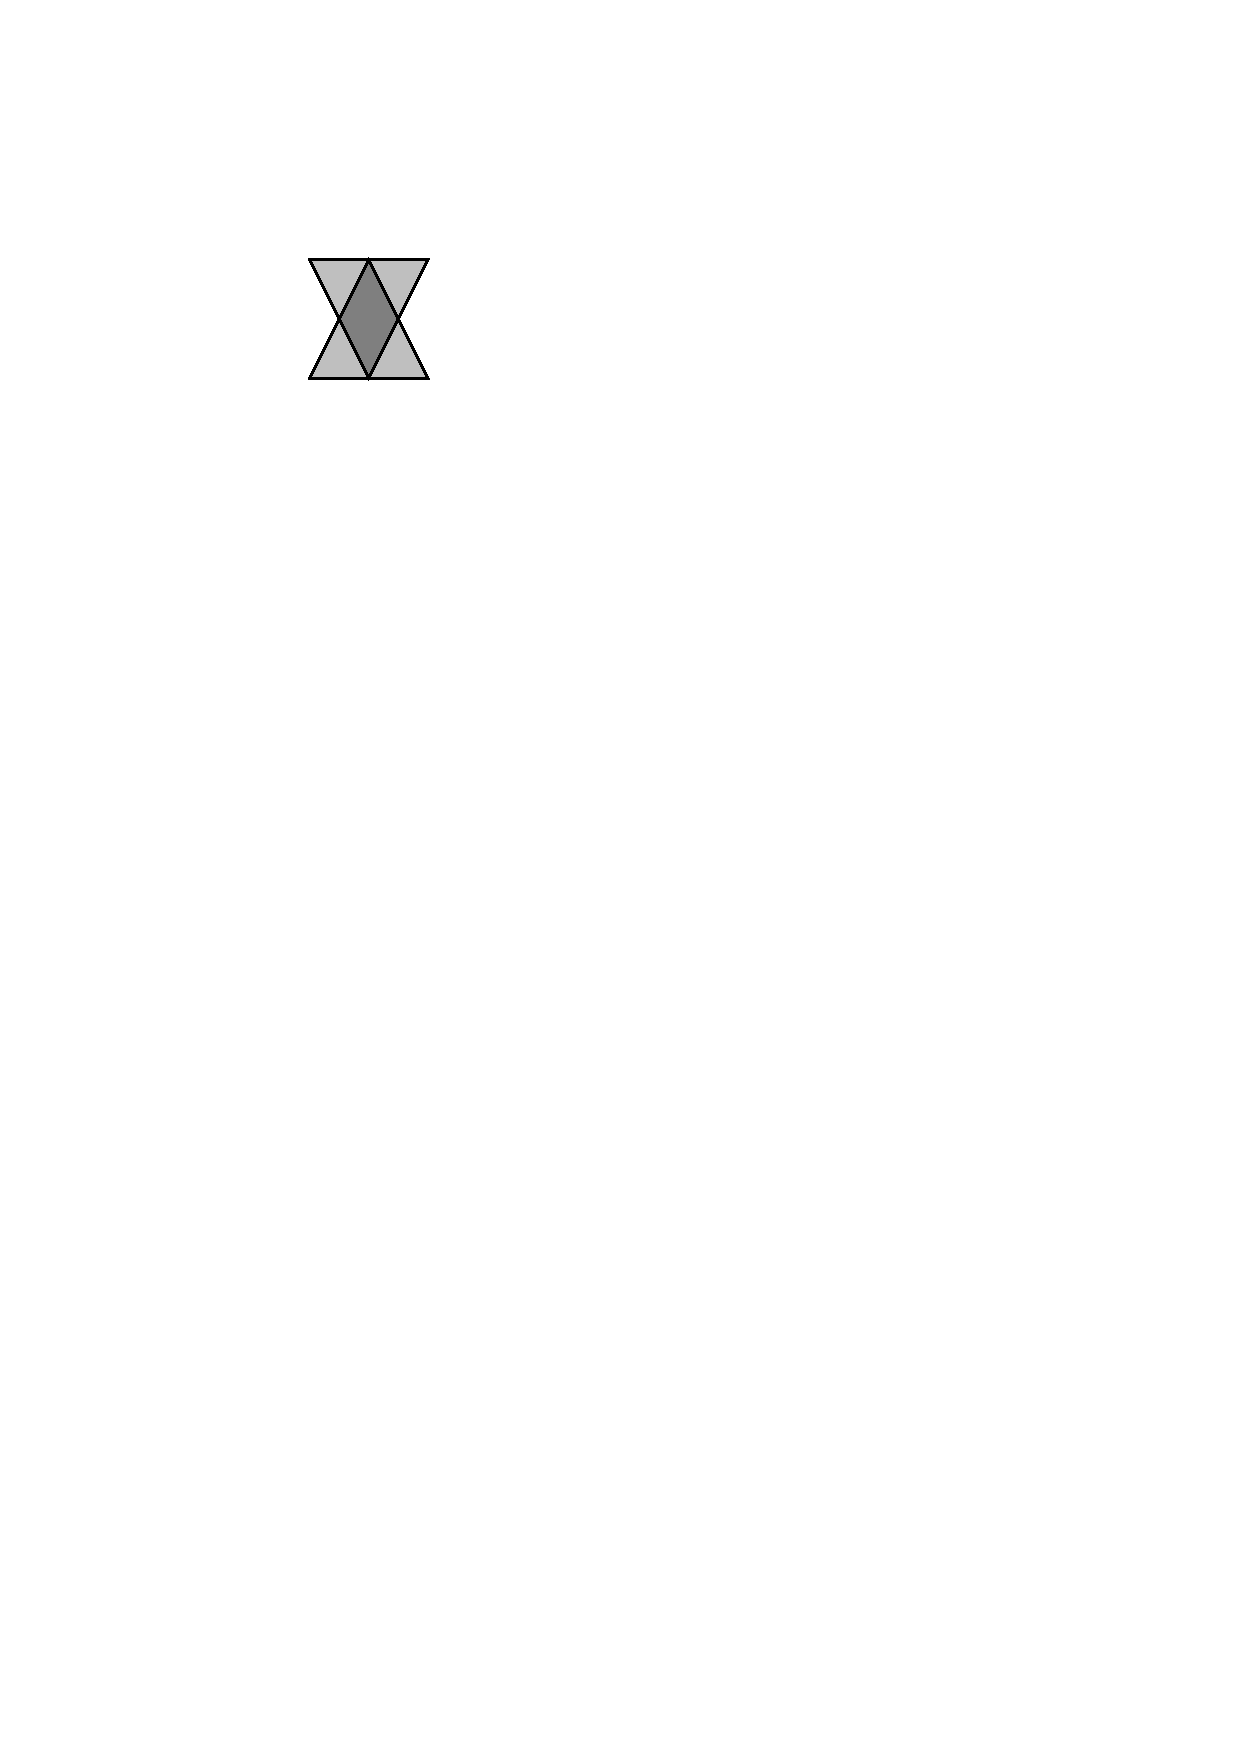
\includegraphics{Boolean_set_operations_2/fig/triangles}
    \end{center}
  \end{minipage}
}

\ccIncludeExampleCode{Boolean_set_operations_2/do_intersect.cpp}

% ----------------------------------
\subsection{Polygons with Holes\label{bso_ssec:polygons_with_holes}}
% ----------------------------------

\begin{figure}[!htp]
\begin{ccTexOnly}
  \begin{center}
  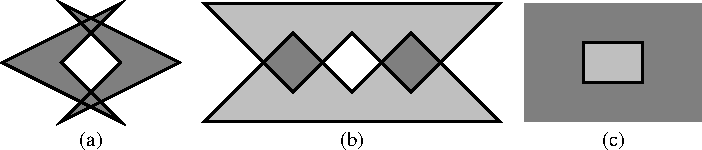
\includegraphics{Boolean_set_operations_2/fig/simple}
  \end{center}
\end{ccTexOnly}
\label{fig:simple}
\begin{ccHtmlOnly}
  <p><center>
    <img src="./fig/simple.gif" border=0 alt="Operations on 
    simple polygons">
  </center>
\end{ccHtmlOnly}
\caption{Operations on simple polygons. (a)~The union of two
polygons, resulting in a point set whose outer boundary is defined by
a simple polygon and contains a polygonal hole in its interior. (b)~The
intersection (darkly shaded) of two polygons (lightly shaded), resulting
in two disjoint polygons. (c)~The complement (darkly shaded) of a
simple polygon (lightly shaded).} 
\end{figure}

In many cases a binary operation that operates on two simple
polygons that have no holes may result in a set of polygons that
contain holes in their interior (see Figure~\ref{fig:simple}~(a)), 
or a set of disjoint polygons (see Figure~\ref{fig:simple}~(b); a similar
set may result from the union, or the symmetric difference, of two disjoint
polygons). Moreover, the complement of a simple polygon is an unbounded set
that contains a hole; see Figure~\ref{fig:simple}~(c).

Regular sets are closed under regularized Boolean set-operations.
These operations accept as input, and may result as output, polygons
with holes. 
A {\em polygon with holes} represents a point set that may
be bounded or unbounded. In case of a bounded set, its {\em outer
boundary} is represented as a relatively simple (but not necessarily simple) polygon, whose vertices are oriented in a counterclockwise
order around the interior of the set. In addition, the set may contain
{\em holes}, where each hole is represented as a simple
polygon, whose vertices are oriented in a clockwise order around the
interior of the hole. Note that an unbounded polygon without holes
spans the entire plane. Vertices of holes may coincide with vertices
of the boundary; see below for an example. 

A point set represented by a polygon with holes is considered to be
closed. Therefore, the boundaries of the holes are parts of the set
(and not part of the holes).
The exact definition of the obtained polygon with holes as a result of
a Boolean set-operation or a sequence of such operations is closely
related to the definition of regularized Boolean set-operations, being
the closure of the interior of the corresponding ordinary operation as
explained next.
\newpage
\lcTex{%
  \setlength{\BooleanSetOpsWidthRight}{1.4cm}
  \setlength{\BooleanSetOpsWidthLeft}{\BooleanSetOpsWidthLineReal}
  \addtolength{\BooleanSetOpsWidthLeft}{-\BooleanSetOpsWidthRight}
  \begin{minipage}{\BooleanSetOpsWidthLeft}
}
\label{fig:unique}
\begin{ccHtmlOnly}
  <img src="./fig/unique.gif" border=0 alt="Unique" align=right>
\end{ccHtmlOnly}
Consider, for example, the regular set depicted on the right, which is
the result of the union of three small triangles translated
appropriately. Alternatively, the same set can be reached by taking
the \ccHtmlNoLinksFrom{difference} between a large triangle and a small
upside-down triangle. In general, there are many ways to arrive at 
a particular point set. However, the set of polygons with holes
obtained through the application of any sequence of operations is
unique. The set depicted on the right is represented as a single
polygon having a triangular outer boundary with a single triangular
hole in its interior --- and not as three triangles that have no holes
at all. As a general rule, if two point sets are connected, then they
belong to the same polygon with holes.
\lcTex{%
  \end{minipage}\hspace{\BooleanSetOpsMinipageSpace}
  \begin{minipage}{\BooleanSetOpsWidthRight}
    \begin{center}
    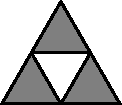
\includegraphics{Boolean_set_operations_2/fig/unique}
    \end{center}
  \end{minipage}
}

The class template \ccc{Polygon_with_holes_2<Kernel,Container>}
represents polygons with holes as described above, where the outer
boundary and the hole boundaries are realized as
\ccc{Polygon_2<Kernel,Container>} objects. Given an instance $P$ of
the \ccc{Polygon_with_holes_2} class, you can use the predicate
\ccc{is_unbounded()} to check whether $P$ is a unbounded set. If it is
bounded, you can obtain the counterclockwise-oriented polygon that
represents its outer boundary through the member function
\ccc{outer_boundary()}. You can also traverse the holes of $P$ through
\ccc{holes_begin()} and \ccc{holes_end()}. The two functions return
iterators of the nested type
\ccc{Polygon_with_holes_2::Hole_const_iterator} that  
defines the valid range of $P$'s holes. The value type of this
iterator is \ccc{Polygon_2}.

The following function demonstrates how to traverse a polygon with holes.
It accepts a \ccc{Polygon_with_holes_2} object and uses the auxiliary
function \ccc{print_polygon()} to prints all its components in a readable
format:
\begin{alltt}
template<class Kernel, class Container>
void print_polygon_with_holes(const CGAL::Polygon_with_holes_2<Kernel, Container> & pwh)
\{
  if (! pwh.is_unbounded()) \{
    std::cout << "\{ Outer boundary = "; 
    print_polygon (pwh.outer_boundary());
  \}
  else
    std::cout << "\{ Unbounded polygon." << std::endl;

  typename CGAL::Polygon_with_holes_2<Kernel,Container>::Hole_const_iterator hit;
  unsigned int k = 1;

  std::cout << "  " << pwh.number_of_holes() << " holes:" << std::endl;
  for (hit = pwh.holes_begin(); hit != pwh.holes_end(); ++hit, ++k) \{
    std::cout << "    Hole #" << k << " = ";
    print_polygon (*hit);
  \}
  std::cout << " \}" << std::endl;
\}
\end{alltt}

The simple versions of the free functions mentioned therefore
accept two \ccc{Polygon_2} object $P$ and $Q$ as their input, while
their output is given using polygon with holes instances:
\begin{itemize}
\item The complement of a simple polygon $P$ is always an unbounded set
with a single polygonal hole. The function \ccc{complement(P)} therefore
returns a polygon-with-holes object that represents the complement of $P$.
\item The union of two polygons $P$ and $Q$ is always a single connected
set, unless of course the two input polygons are completely disjoint. In
the latter case $P \cup Q$ trivially consists of the two input polygons.
The free function \ccc{join(P, Q, R)} therefore returns a Boolean value
indicating whether $P \cap Q \neq \emptyset$. If the two polygons are not
disjoint, it assigns the polygon with holes object $R$ (which it
accepts by reference) with the union of the regularized union operation
$P \cup Q$.
\item The other three functions, namely \ccc{intersection(P, Q, oi)}, 
\ccc{difference(P, Q, oi)} and \ccc{symmetric_difference(P, Q, oi)}, all
have a similar interface. As the result of these operation may consist
of several disconnected components, they all accept an output iterator
\ccc{oi}, whose value type is \ccc{Polygon_with_holes_2}, and adds the
output polygons to its associated container.
\end{itemize}

% ~~~~~~~~~~~~~~~~~~~~~~~~~~~~~~~~~~~~~~~~~~~~~~~~~~~~~~~~~~~~~~~~~~
\subsubsection{Example --- Joining and Intersecting Simple Polygons\label{bso_sssec:ex_simple_bops}}
% ~~~~~~~~~~~~~~~~~~~~~~~~~~~~~~~~~~~~~~~~~~~~~~~~~~~~~~~~~~~~~~~~~~

The following example demonstrates the usage of the free functions
\ccc{join()} and \ccc{intersect()} for computing the union and the
intersection of the two simple polygons depicted in
Figure~\ref{fig:simple}~(b). The example uses the auxiliary function
\ccc{print_polygon_with_holes()} listed above, which is located in
the header file \ccc{print_utils.h} under the examples folder.

\ccIncludeExampleCode{Boolean_set_operations_2/simple_join_intersect.cpp}

% ~~~~~~~~~~~~~~~~~~~~~~~~~~~~~~~~~~~~~~~~~~~~~~~
\subsubsection{Operations on Polygons with Holes\label{bso_sssec:pwh_bops}}
% ~~~~~~~~~~~~~~~~~~~~~~~~~~~~~~~~~~~~~~~~~~~~~~~
We have demonstrated that free functions that perform boolean set operations on simple polygons may output polygons with holes. In addition to these functions, the Boolean set-operations package provides the following overridden free functions that accept
\ccc{General_polygon_with_holes_2} objects as their input - 
%Having introduced polygons with holes and explained how the free functions
%output such objects, it is only natural to perform operations on sets that
%are represented as polygon with holes, rather than simple polygons.
%Indeed, the Boolean set-operations package provides overriden free functions
\ccc{complement()}, \ccc{intersection()}, \ccc{join()}, \ccc{difference()},
\ccc{symmetric_difference()} and \ccc{do_intersect()}  The prototypes of
most functions is the same as of their simpler counterparts that operate
on simple polygons. The only exception is \ccc{complement(P, oi)}, which
outputs a range of polygons with holes that represents the complement
of the polygon with holes $P$.

\lcTex{%
  \setlength{\BooleanSetOpsWidthRight}{2.5cm}
  \setlength{\BooleanSetOpsWidthLeft}{\BooleanSetOpsWidthLineReal}
  \addtolength{\BooleanSetOpsWidthLeft}{-\BooleanSetOpsWidthRight}
  \begin{minipage}{\BooleanSetOpsWidthLeft}
}
\label{fig:sym_diff}
\begin{ccHtmlOnly}
  <img src="./fig/symm_diff.gif" border=0 alt="Unique" align=right>
\end{ccHtmlOnly}
The following example demonstrates how to compute the symmetric
difference between two sets that contain holes. Each set is a
rectangle that contains a rectangular hole in its interior, such that
the symmetric difference between the two sets is a single polygon that
contains of five holes:
\lcTex{%
  \end{minipage}\hspace{\BooleanSetOpsMinipageSpace}
  \begin{minipage}{\BooleanSetOpsWidthRight}
    \begin{center}
    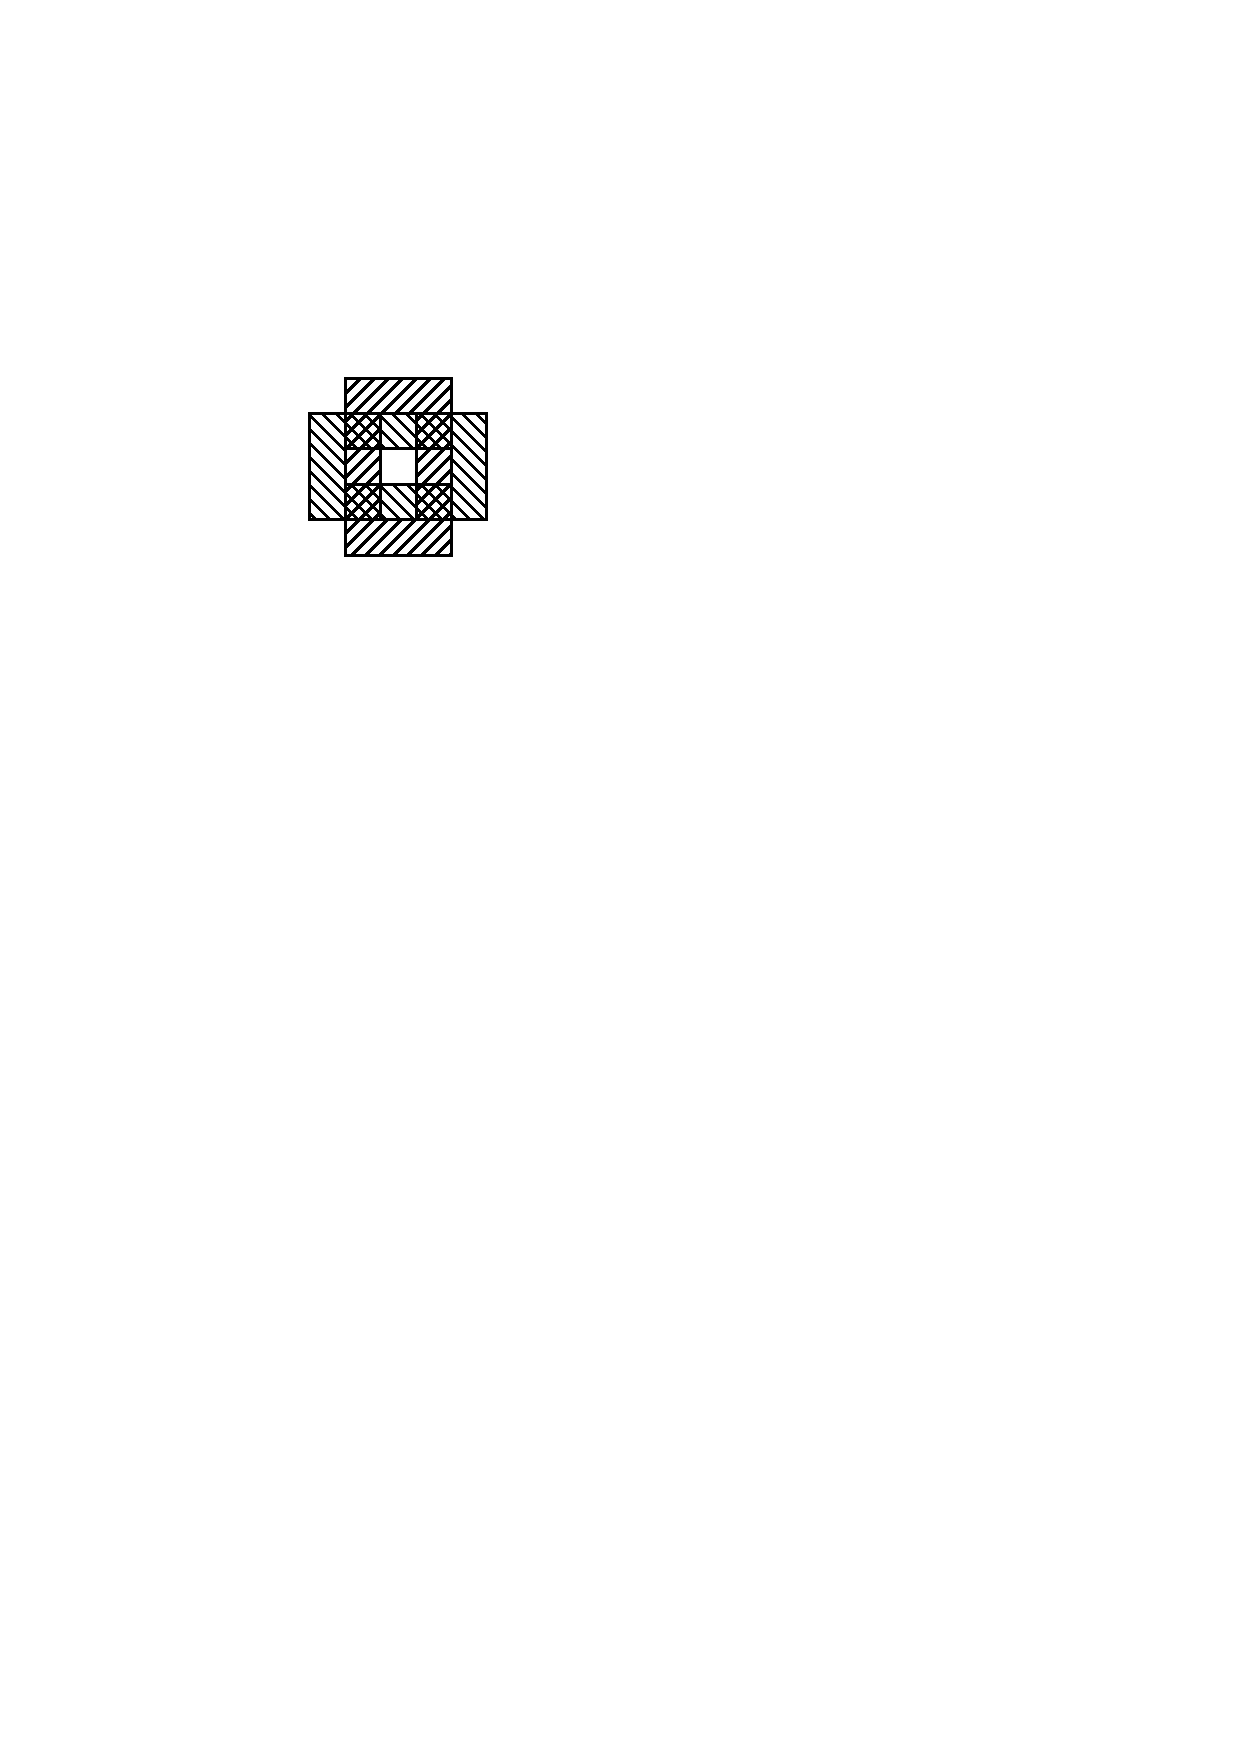
\includegraphics{Boolean_set_operations_2/fig/symm_diff}
    \end{center}
  \end{minipage}
}

\ccIncludeExampleCode{Boolean_set_operations_2/symmetric_difference.cpp}

In some cases it is convenient to connect the outer boundary of a
polygon with holes with the holes inside it. The
function \ccc{connect_holes()} accepts a polygon with
holes, and connects the topmost vertex in each hole with the polygon
feature located directly above it (a vertex or an edge of the outer
boundary, or of another hole). It produces an output sequence of
points that match the traversal of all vertices in the connected
polygon (note that there are additional vertices, induced by the
vertical walls).

\ccIncludeExampleCode{Boolean_set_operations_2/connect_polygon.cpp}

% ------------------------------------
\subsection{Operating on Polygon Sets\label{bso_ssec:main_component}}
% ------------------------------------

We argue that the result of a regularized operations on two polygons
(or polygons with holes) $P$ and $Q$ is typically a collection of
several disconnected polygons with holes. It is only natural to
represent such a collection in terms of a class, making it possible to
operate on the set resulting from computing, for example, $P \setminus
Q$.

A central component in the Boolean set-operations package is the
\ccc{Polygon_set_2<Kernel, Container, Dcel>} class-template. An instance of 
this class represents a point set formed by the collection of several 
disconnected polygons with holes. It employs the \ccc{Arrangement_2} class 
to represent this point set in the plane as a planar arrangement; see 
Chapter~\ref{chapterArrangement_on_surface_2}. The instantiated \ccc{Dcel}
type is used to represent the underlying internal arrangement. It must model
the concept \ccc{GeneralPolygonSetDcel}, and defaults to \ccc{Gps_default_dcel}.
You can override this default, with a different {\sc Dcel} class, typically
an extension of the default. Overriding the default is necessary only if 
you intend to obtain the underlying internal arrangement and process it further.

An instance $S$ of a \ccc{Polygon_set_2} class usually represents
the result of a sequence of operations that were applied on some input
polygons. The representation of $S$ is unique, regardless of the particular
sequence of operations that were applied in order to arrive at it.

In addition, a polygon-set object can be constructed from a single
polygon object or from a polygon-with-holes object. Once constructed,
it is possible to insert new polygons (or polygons with holes)
into the set using the \ccc{insert()} method, as long as the inserted
polygons and the existing polygons in the set are disjoint. 
The \ccc{Polygon_set_2} class also provides access functions for
accessing the polygons with holes it contains, and a few queries. The
most important query is \ccc{S.oriented_side(q)}, which determined
whether the query point $q$ is contained in the interior of the set
$S$, lies on the boundary of the set, or neither.

The \ccc{General_polygon_set_2} class defines the predicate
\ccc{do_intersect()} and the methods \ccc{complement()}, \ccc{intersection()},
\ccc{join()}, \ccc{difference()} and \ccc{symmetric_difference()} as member
functions. The operands to these functions may be simple polygons 
(\ccc{Polygon_2} object), polygons with holes
(\ccc{General_polygon_with_holes_2} objects), or polygon sets
(\ccc{General_polygon_set_2} objects). Thus, each of the function
mentioned above is actually realized by a set overriding member
functions.

Member functions of the \ccc{General_polygon_set_2} that perform
Boolean set-operations come in two flavors: for example, \ccc{S.join(P, Q)}
computes the union of $P$ and $Q$ and assigned the result to $S$, while
\ccc{S.join(P)} performs the operation $S \longleftarrow S \cup P$.
Similarly, \ccc{S.complement(P)} sets $S$ to be the complement of $P$,
while $S.complement()$ simply negates the set $S$.

% ~~~~~~~~~~~~~~~~~~~~~~~~~~~~~~~~~~~~~~~~~~
\subsubsection{A Sequence of Set Operations\label{bso_sssec:sequence}}
% ~~~~~~~~~~~~~~~~~~~~~~~~~~~~~~~~~~~~~~~~~~

The free functions reviewed in Section~\ref{bso_ssec:polygons_with_holes}
serve as a wrapper for the polygon-set class, and are only provided for
convenience. A typical such function constructs a pair of
\ccc{General_polygon_set_2} objects, invokes the appropriate method to
apply the desired Boolean operation, and transforms the resulting
polygon set to the required output format. Thus, when several
operations are performed in a sequence, it is much more efficient to
use the member functions of the \ccc{General_polygon_set_2} type
directly, as the extraction of the polygons from the internal
representation for some operation, and the reconstruction of the
internal representation for the succeeding operation could be time
consuming.

\lcTex{%
  \setlength{\BooleanSetOpsWidthRight}{2.3cm}
  \setlength{\BooleanSetOpsWidthLeft}{\BooleanSetOpsWidthLineReal}
  \addtolength{\BooleanSetOpsWidthLeft}{-\BooleanSetOpsWidthRight}
  \begin{minipage}{\BooleanSetOpsWidthLeft}
}
\label{fig:sequence}
\begin{ccHtmlOnly}
  <p><center>
    <img src="./fig/sequence.gif" border=0 alt="A sequence of operation" align=right>
  </center>
\end{ccHtmlOnly}
The next example performs a sequence of three Boolean set-operations.
First, it computes the union of two simple polygons depicted in
Figure~\ref{fig:simple}~(a). It then computes the complement of the result
of the union operation. Finally, it computes the intersection of the result
of the complement operation with a rectangle, confining the final result to 
the area of the rectangle. The resulting set $S$ is comprised of two
components: a polygon with a hole, and a simple polygon contained in the
interior of this hole.
\lcTex{%
  \end{minipage}\hspace{\BooleanSetOpsMinipageSpace}
  \begin{minipage}{\BooleanSetOpsWidthRight}
    \begin{center}
    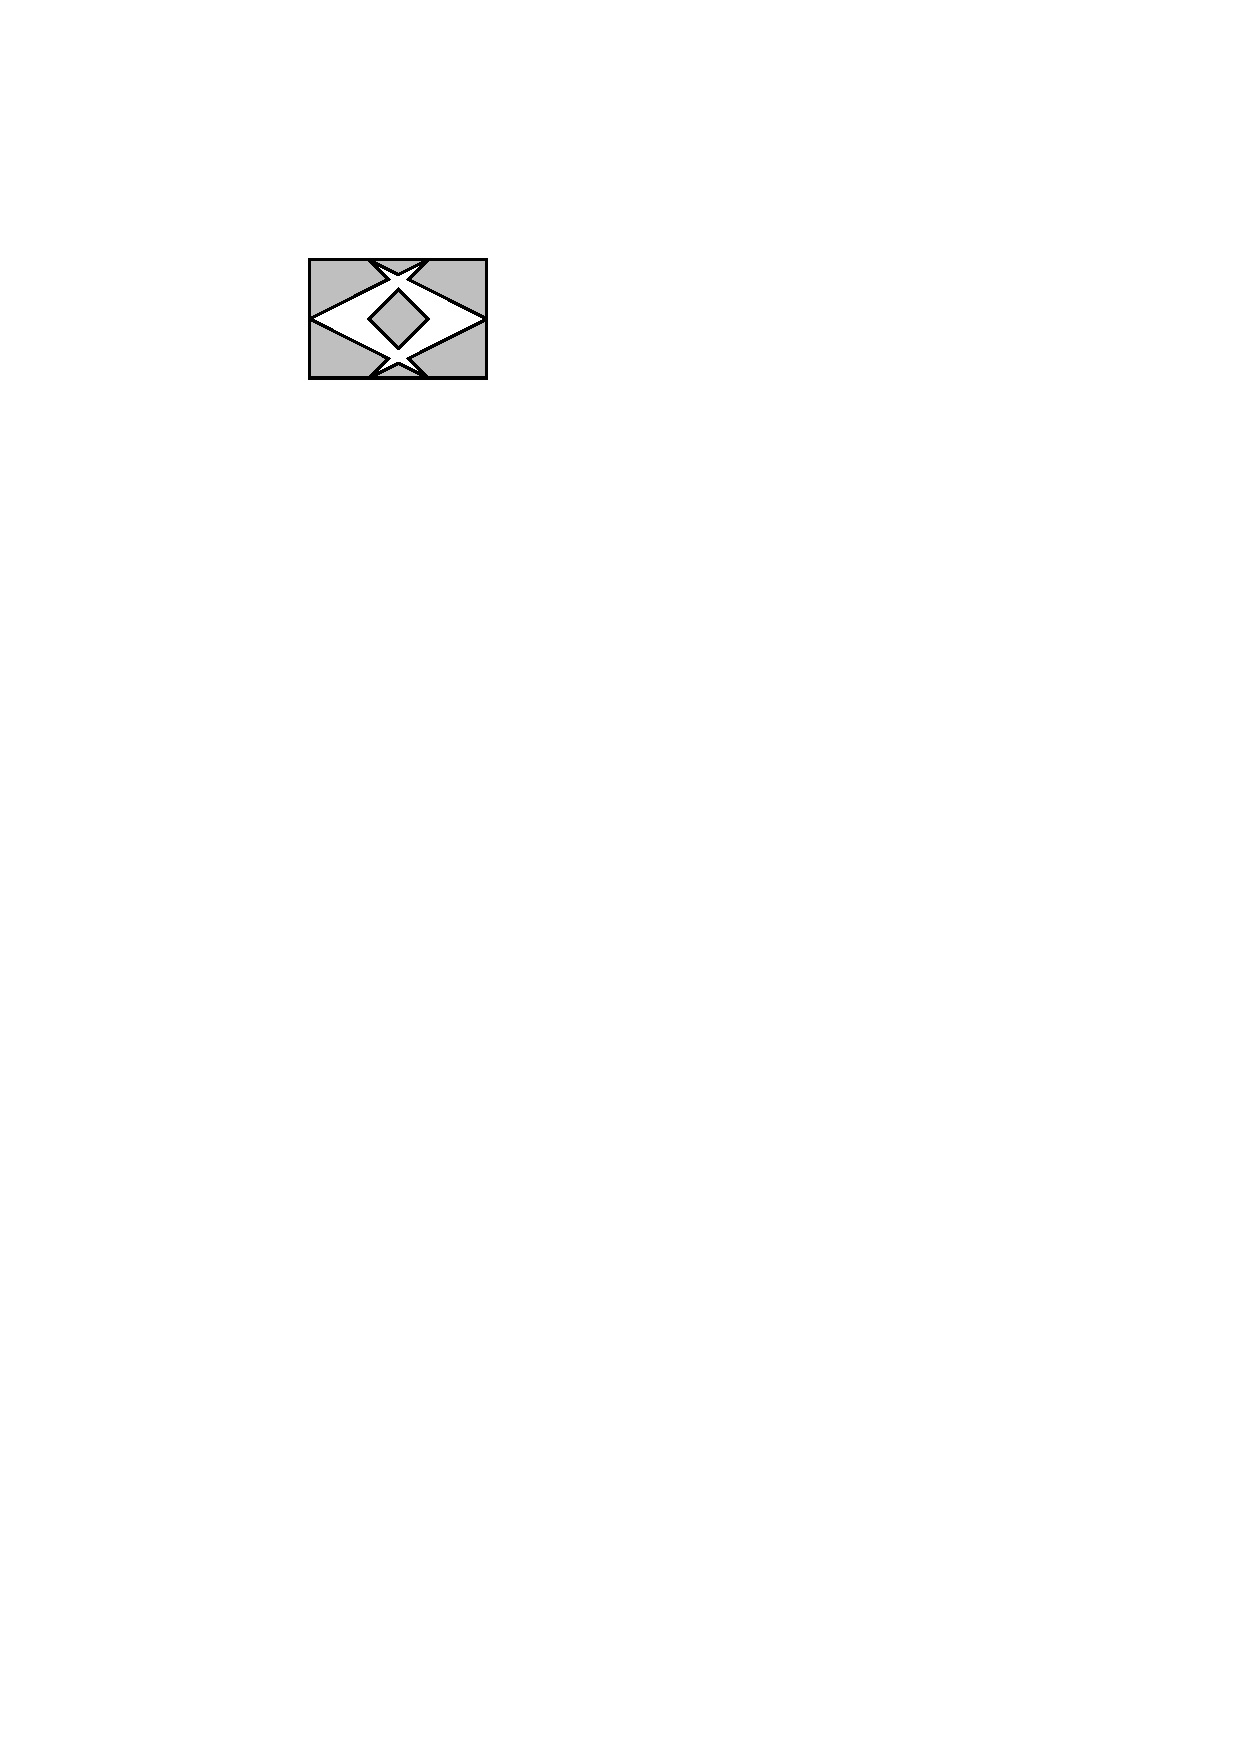
\includegraphics{Boolean_set_operations_2/fig/sequence}
    \end{center}
  \end{minipage}
  \vspace{2pt}
}

\ccIncludeExampleCode{Boolean_set_operations_2/sequence.cpp}

% ~~~~~~~~~~~~~~~~~~~~~~~~~~~~~~~~~~~~~~~~~~~~~~~~~
\subsubsection{Inserting Non Intersecting Polygons\label{bso_ssec:insert_ni}}
% ~~~~~~~~~~~~~~~~~~~~~~~~~~~~~~~~~~~~~~~~~~~~~~~~~

If you want to compute the union of a polygon $P$ ($P$ may be a simple
polygon or a polygon-with-holes object) with a general-polygon set
$R$, and store the result in $R$, you can construct a polygon set
$S(P)$, and apply the {\em union} operation as follows:
\begin{alltt}
  General_polygon_2 S (P);
  R.join (S);
\end{alltt}

As a matter of fact, you can apply the union operation directly:
\begin{alltt}
  R.join (P);
\end{alltt}

However, if you know that the polygon does not intersect any one of the
polygons represented by $R$, you can use the more efficient method
\ccc{insert()}:
\begin{alltt}
  R.insert (P);
\end{alltt}

As \ccc{insert()} assumes that $P \cap R = \emptyset$, it does not try to
compute intersections between the boundaries of $P$ and of $R$. This
fact significantly speeds up the insertion process in comparison with the
insertion of a non-disjoint polygon that intersects $R$.

The \ccc{insert()} function is also overloaded, so it can also accept a
range of polygons. When a range of polygons are inserted into a
polygon set $S$, all the polygons in the range and the polygons represented 
by $S$ must be pairwise disjoint in their interiors.

% -------------------------------------------
\subsection{Performing Aggregated Operations\label{bso_ssec:agg_ops}}
% -------------------------------------------

There are a few options to compute the union of a set of polygons
$P_1, \ldots P_m$. You can do it incrementally as follows. At each step
compute the union of $S_{k-1} = \bigcup_{i=1}^{k-1}{P_i}$ 
with $P_{k}$ and obtain $S_k$. Namely, if the polygon set is given
as a pair of iterator \ccc{[begin, end)}, the following loop computes
their union in $S$.
\begin{alltt}
  InputIterator iter = begin;
  Polygon_set_2 S (*iter);

  while (++iter != end) \{
    S.join (*iter);
    ++iter;
  \}
\end{alltt}  
A second option is to use a divide-and-conquer approach. You bisect
the set of polygons into two sets. Compute the union of each set
recursively and obtain the partial results in $S_1$ and $S_2$, and
finally, you compute the union $S_1 \cup S_2$. However, the union
operation can be done more efficiently for sparse polygons, having
a relatively small number of intersections, using a third option that
simultaneously computes the union of all polygons. This is done by 
constructing a planar arrangement of all input polygons, utilizing the
sweep-line algorithm, then extracting the result from the
arrangement. Similarly, it is also possible to aggregately compute the
intersection $\bigcap_{i=1}^{m}{P_i}$ of a set of input polygons.

Our package provides the free overloaded functions \ccc{join()} and
\ccc{intersect()} that aggregately compute the union and the intersection
of a range of input polygons. There is no restriction on the polygons in the
range --- naturally, they may intersect each other.
The package provides the overloaded free function 
\ccc{do_intersect(begin, end)} that determines whether the polygons in the
range defined by the two input iterators \ccc{[begin, end)} intersect.

The class \ccc{General_polygon_set_2} also provides equivalent member
functions that aggragately operate on a range of input polygons or
polygons with holes. When such a member function is called, the general 
polygons represented by the current object are considered operands as 
well. Thus, you can easily compute the union of our polygon range as
follows:
\begin{alltt}
  Polygon_set_2 S;
  S.join (begin, end);
\end{alltt} 
